%-------------------------------------------------------------------------
%   PACKAGES AND OTHER DOCUMENT CONFIG
%-------------------------------------------------------------------------

\documentclass[11pt]{article}

%----------------------------------------------------------------------------------------------
%   PACKAGES AND CONFIGURATIONS 
%----------------------------------------------------------------------------------------------

\usepackage{lastpage}
\usepackage{hyperref}
\usepackage{graphicx}
\usepackage{pgfplots}
\pgfplotsset{compat=1.17}
\usepackage{xcolor}
\usepackage{amsmath}
\usepackage{bussproofs}
\usepackage{amssymb}
\usepackage{amsfonts}
\usepackage{graphicx}
\usepackage{booktabs}
\usepackage{listing}
\usepackage{etoolbox}
\usepackage{latexsym}
\usepackage{listings}
\usepackage[utf8]{inputenc}
\usepackage{caption}
\graphicspath{{./img}}

\DeclareCaptionFont{white}{\color{white}}
\DeclareCaptionFormat{listing}{%
  \parbox{\textwidth}{\colorbox{gray}{\parbox{\textwidth}{#1#2#3}}\vskip-4pt}}
\captionsetup[lstlisting]{format=listing,labelfont=white,textfont=white}
\lstset{frame=lrb,xleftmargin=\fboxsep,xrightmargin=-\fboxsep}

%-----------------------------------------------------------------------------------------------
%   MARGINS
%-----------------------------------------------------------------------------------------------

\usepackage{geometry}
\geometry{
    paper=a4paper,
    top=3cm,
    bottom=3cm,
    left=2.5cm,
    right=2.5cm,
    headheight=14pt,
    footskip=1.4cm,
    headsep=1.2cm,
}

%-----------------------------------------------------------------------------------------------
%   FONT
%-----------------------------------------------------------------------------------------------

\usepackage[utf8]{inputenc}
\usepackage[T1]{fontenc}

\usepackage[sfdefault,light]{roboto}

%-----------------------------------------------------------------------------------------------
%   HEADER AND FOOTER   
%-----------------------------------------------------------------------------------------------

\usepackage{fancyhdr}
\pagestyle{fancy}

\lhead{\small\classHomework\ifdef{\className}{\ (\className):}{}\ \homeworkTitle}
\chead{}
\rhead{\small\ifdef{\authorName}{\authorName}{\ifdef{dueDate}{Due\ \dueDate}{}}}

\lfoot{}
\cfoot{\small Page\ \thepage\ of\ \pageref{LastPage}}
\rfoot{
\includegraphics[scale=0.06]{logo-unige.png}}

\renewcommand\headrulewidth{0.5pt}

%-------------------------------------------------------------------------------------------------
%   TITLE PAGE
%-------------------------------------------------------------------------------------------------

\author{\textbf{\authorName}}
\date{}

\title{
    \thispagestyle{empty}
    \vspace{0.2\textheight}
    \textbf{\classHomework:\ \homeworkTitle}\\[-4pt]
    \ifdef{\classHomework}{{\small Due\ on\ \dueDate}\\}{}
    \ifdef{\className}{{\large \textit{\className}}}{}
    \vspace{0.32\textheight}

    
\includegraphics[scale=0.2]{logo-unige.png}
}


%-------------------------------------------------------------------------
%   HOMEWORK INFORMATION
%-------------------------------------------------------------------------

\newcommand{\classHomework}{13X007}
\newcommand{\homeworkTitle}{Assignment\ \#3}
\newcommand{\authorName}{CHRISTOFOROU Anthony}
\newcommand{\className}{Parallelism}
\newcommand{\dueDate}{08.11.2023}

%-------------------------------------------------------------------------

\begin{document}
    
    \maketitle
    \thispagestyle{empty}
    \newpage

    \begin{abstract}
    This report delves into the implementation and analysis of a parallelized C++ program, designed for calculating the value of $\pi$ using the Riemann sum method, with a focus on employing OpenMP for efficient parallel computation. The report elaborates on the theoretical foundation, challenges, performance results, and potential improvements in the context of parallel computing and numerical methods.
    \end{abstract}

    \tableofcontents
    
    \newpage
    
    \section{Introduction}
    The calculation of $\pi$ using numerical methods is a classic problem in computational mathematics. This report presents a parallelized approach using the Riemann sum method in C++, leveraging the OpenMP framework for enhanced computational performance. The objective is to demonstrate efficient parallel computing techniques in approximating mathematical constants and to analyze the scalability and accuracy of such methods.

    \section{Theoretical Background}
    \subsection{Riemann Sum}
    \begin{figure}[h]
        \centering
        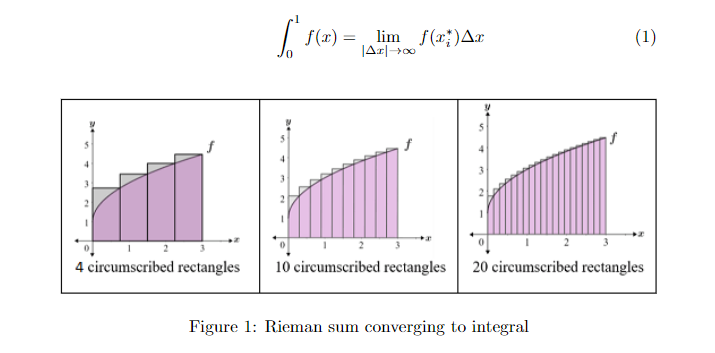
\includegraphics[width=0.8\textwidth]{img/riemansum.png}
        \label{fig:riemann_sum}
    \end{figure}
    The Riemann sum is a fundamental concept for approximating the definite integral of a function. It involves summing the areas of rectangles under a curve, providing an approximation of the integral. The basic formula for a Riemann sum is:
    \[ S = \sum_{i=1}^{n} f(x_i) \Delta x \]
    where $\Delta x$ is the width of each sub-interval, and $f(x_i)$ is the function value at a chosen point $x_i$ in the $i$-th sub-interval.

    \subsection{Integration of $f(x) = \frac{1}{1+x^2}$}
    The function $f(x) = \frac{1}{1+x^2}$, when integrated over the interval [0, 1], yields $\pi/4$. Thus, the area under this curve approximates $\pi/4$, and multiplying the result by 4 gives an approximation of $\pi$.

    \section{Implementation}
    The program calculates the area under the curve $f(x) = \frac{1}{1+x^2}$ by dividing the interval [0, 1] into $10^8$ rectangles and summing their areas, using the midpoint of each rectangle to evaluate the function. 

    \subsection{Code Explanation}
    \begin{verbatim}
    double sum = 0.0;
    double step = 1.0 / (double)num_steps;
    #pragma omp parallel for reduction(+:sum)
    for (int i = 0; i < num_steps; i++) {
        double x = (i + 0.5) * step;
        sum += 4.0 / (1.0 + x * x);
    }
    double pi = step * sum;
    \end{verbatim}
    The code employs OpenMP directives for parallelizing the loop that calculates the Riemann sum. The `reduction(+:sum)` clause ensures thread-safe addition to the variable `sum`.

    \section{Performance Results and Analysis}
    \subsection{Execution Times}
    The program's performance was evaluated with varying numbers of threads. The execution times and the calculated values of $\pi$ were recorded, showing a decrease in computation time with an increase in threads, up to a certain point.

    \subsection{Output Analysis}
    The output of the program with different thread counts is as follows:
    \begin{verbatim}
    Threads: 2, Time: 0.0964905 seconds, pi: 3.14159
    Threads: 4, Time: 0.0670324 seconds, pi: 3.14159
    ...
    Threads: 256, Time: 0.0422394 seconds, pi: 3.14159
    \end{verbatim}
    These results indicate that the parallelized implementation efficiently reduces computation time, especially for lower thread counts. However, beyond a certain number of threads, the improvement in performance becomes less significant.

    \section{Challenges and Limitations}
    The implementation, while effective, faces certain challenges:
    \begin{itemize}
        \item \textbf{Scalability}: The diminishing returns in performance improvement with higher thread counts highlight the scalability limitations due to overheads in thread management and synchronization.
        \item \textbf{Accuracy}: The accuracy of the Riemann sum approach depends on the number of rectangles; more rectangles generally mean better accuracy but at the cost of increased computation time.
        \item \textbf{Hardware Constraints}: The performance also depends on the hardware capabilities, particularly the number of available processor cores.
    \end{itemize}

    \section{Conclusion}
    This report demonstrates the application of parallel computing in approximating $\pi$ using the Riemann sum method. By employing OpenMP, the program achieves significant improvements in computation time, showcasing the potential of parallel programming in numerical methods. Future work could explore alternative approaches and optimizations to overcome scalability and accuracy limitations.

\end{document}
